\chapter{Methodology}

This chapter describes the adopted method for collecting relevant constraints, relating these to the common security-goals of CIAA, and later mapping them to functionality within ArchUnit. Second, this chapter presents the validation plan for expressing security constraints with ArchUnit (as is) by means of an illustration and for expressing additional constraints by means of a controlled experiment.

\section{Data collection}\label{sec:data_collection}

The relevance of the security architectural constraints included in the study was ensured by performing a review of security measures and common weaknesses and compiling the result to a list of constraints. Completeness was not the primary goal of the review, but rather to provide a set of constraints derived from previous knowledge. Presented below are the three sources used to form the final list. 

\textbf{CAWE catalog:}
The Common Architectural Weakness Enumeration catalog \cite{santos_catalog_2017} details 224 common weaknesses in security architectures. Each entry has a description of the weakness and exemplifications of how it could manifest itself in the source code, when applicable. In some entries, there are recommendations on what techniques can be used to detect the weakness, along with mitigation strategies.

\textbf{Security patterns:}
Similar to the usage of general design patterns made famous in \cite{gamma_design_1995}, security patterns provide a reusable and domain-independent solution to a known problem. More specifically, this study focused on security patterns for the design phase, as defined in \cite{yoshioka_survey_2008}. While the security pattern repository\footnote{http://sefm.cs.utsa.edu/repository/} lists over 170 security patterns, not all are provided with sufficient detail or at the appropriate level of abstraction. As a result, the report by Scandariato et al. \cite{scandariato_system_2006}  which provides a filtered list of patterns.


\textbf{Security rules:} \label{subsec:security_rules}
Architectural security rules constrain the implementation of a system while being less solution-oriented compared to security patterns. Eden and Kazman differentiate architectural security rules from those defined on a level of source code based on two criteria, locality and intension/extension \cite{eden_architecture_2003}. Architectural rules are both non-local and intensional, meaning that they affect all or several parts of the system while having \say{infinitely-many possible instances}. In \cite{franch_constraining_2019}, Jasser presents a catalog of architectural security rules. Although the entire catalog of 150 security rules is not yet available, the initial list of 22 included in the paper was used in our study.

\section{Filtering}\label{sec:processing}

%Elaborate. Perhaps explaining how the sources were analyzed. Did you analyse one right after the other, were there iterations, did you meet after each iteration to discuss your findings and synchronize individually derived subset, or did you work together? How many constraints were taken from individual sources, which of those were grouped? What is the proportion of CIAA coverage in the final list (Show CIAA in table 4.2 and show #ID linking the chosen ones from 4.1)? What was the rational for grouping? Perhaps explicitly enumerating  the "rules" you followed for inclusion would be nice (if there are more than two :) ...), e.g.:
%1) only security related architectural constraints were considered
%2) only constraints that can be enforced statically (FYI: prepare for the question, what is an example of a constraint that can not be statically enforced?),
%3) ...
Starting from each of the three sources of architectural constraints described in Section~\ref{sec:data_collection}, the first step of the process, shown in Figure~\ref{fig:mapping_process}, was to select the entries that could be formulated as enforceable constraint in the context of our project. The criteria for inclusion were the following: 

\begin{enumerate}
    \item The entry must be related to the architectural design of a system, i.e., non-local and intensional (as described in section \ref{subsec:security_rules}. \label{criterion_1}
    \item It must be possible to enforce the entry through static analysis. An example on a non enforceable constraint is "No two instances of a microservice are deployed on the same machine", as the number of machines deployed is a dynamic property. \label{criterion_2}
    \item Although somewhat included in the first criterion as it is a local issue, an entry must not relate to the correctness or best practice of the implementation of an algorithm. Examples include the practice of using session tokens with time-limited validity. \label{criterion_3}
    \item The entry must only relate to the system under design, thus ignoring the correctness and security of any external dependencies. An example can be found in SonarQube where the usage of a version of a library with known vulnerabilities is reported as a weakness. \label{criterion_4}
    \item The entry must not be dependent on externally defined data. A common example is that of user permissions where the mapping between a regulated functions and a users rights is performed using an access control list. \label{criterion_5}
    \item Additionally, we deemed measures defined as the absence of certain functionality as less valuable due to the increased difficulty of enforcement \cite{haley_security_2008}.
\end{enumerate}

\begin{figure}
    \centering
    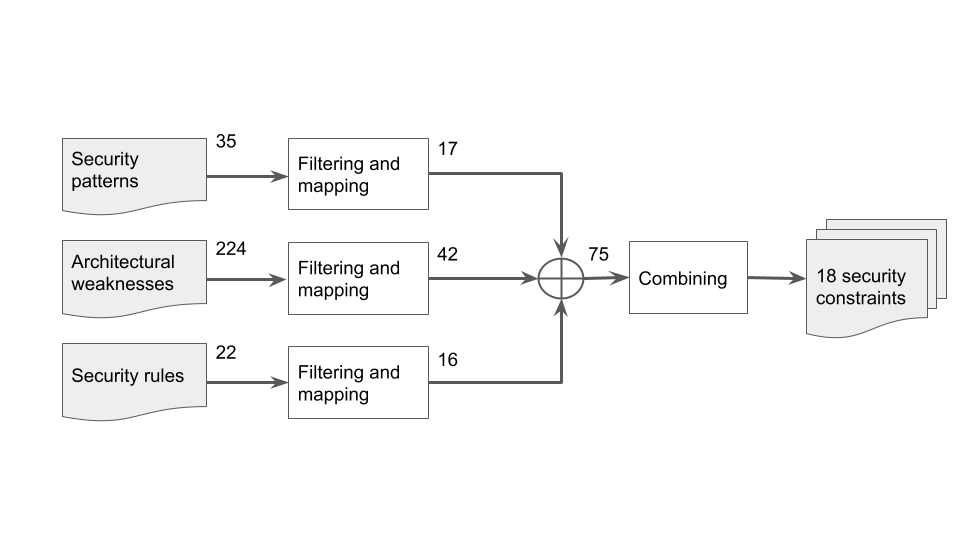
\includegraphics[width=\textwidth]{figure/Half-time presentation.png}
    \caption{Overview of the process of mapping the three sources to constraints}
    \label{fig:mapping_process}
\end{figure}

Previous research on design notations of secure systems have shown a skew towards confidentiality and integrity while having little or no support for availability and accountability. We considered it necessary for the final list of constraints to include all of the security goals. As a consequence, once we had selected the applicable entries, we categorized them according to the security goals of CIAA, ensuring that the final list of constraints covered all security goals. 

The last part of compiling a list of security architectural constraints involved combining the selected entries to remove duplicates and group similar concepts. Duplication involved both a single source having several entries, such as CAWE having input validation weakness for multiple tools and technologies (e.g., SQL, LDAP) and different sources having entries for the same concept, such as the security pattern input guard and the previously mentioned input validation weaknesses. Grouping similar concepts also allowed for the constraints to be more general, thus making them applicable for a broader set of systems. 

\section{Evaluation}\label{sec:evaluation}

The study followed the research design described in \cite{stol_abc_2018} as a "solution-seeking + sample study."  The first part, solution-seeking, covers the overall idea of prosing a solution to an identified problem, namely integrating security architectural constraints within already established testing infrastructure.  The second part, a sample study, aimed to achieve generalizability by composing security architectural constraints that were not tied to a specific domain and later evaluating the performance of the tool when applied to several systems

We evaluated ArchUnit in two ways, comparing it to the two industry used and open-source static analysis tools SonarQube and PMD, as well as a separate analysis focusing solely on ArchUnit. The separation had to be made as an initial assessment of both SonarQube and PMD showed that they could not track information flow. 

In the section to follow, the design of the experiment is described in detail. 

\subsection{Tools used in comparison}\label{sec_tools_used_in_comparison} \todo{fix}
In order to test how reliably SecArchUnit can validate the constraints, we perform a comparison with two static analysis tools widely adopted in industry: SonarQube and PMD.
While these tools have a multitude of built-in rules, none of these rules can be used to enforce the architectural security constraints presented in this thesis. However, both tools are extensible, allowing a developer to define custom rules using their respective APIs.

\todo{describe limitations}
As mentioned in \ref{sec:evaluation}, an initial assessment of the tools determined that constraints one through five are possible to implement and validate using SonarQube and PMD. %describe limitations

Hence, the first five constraints in evaluated SecArchUnit, SonarQube and PMD, whereas the final two constraints are evaluated solely in SecArchUnit.

\subsection{Subjects of analysis} \label{sct:selected-systems}
\todo{describe projects, why they were selected}

Several requirements were formed to guide the selection of projects to be included in the evaluation of our study. While some were necessary due to the languages supported by ArchUnit, others served to decrease the threats to validity. Detailed below is the final list of requirements for inclusion:

\begin{enumerate}
    \item \textbf{The project must be open source}. The static analysis of ArchUnit inherently can not be performed system where the source code is not available.
    \item \textbf{The source code must be written in Java}. As ArchUnit currently does not support any other language, a strict requirement had to be made regarding the langugage. 
    \item \textbf{The project must be previously used in literature concerning security}. Using projects already analyzed in previous litterateur would reduce the bias of the ground truth. 
    \item \textbf{The project must include some form of architectural description}. Architectural description would allow the constraints to be appropriately placed on a system in regards to the security requirements which it has been developed for.
\end{enumerate}

Based on the presented criterion, three systems were selected for the evaluation, JPetStore, ATM Simulation and iTrust. A summary of the characteristics for each system can be sen in table \ref{tab:sample_systems}.

\textbf{JPetStore}, originally designed as an example of how to use the J2EE framework, is built on top of MyBatis 3, Spring and the Stripes framework. The application is a minimal implementation of an online pet store. It has been used both as an industry benchmark application \cite{luo_forepost_2017} and in the context of security analysis \cite{peldszus_secure_2019}

\textbf{ATM Simulator}

\textbf{iTrust}

\begin{table}[]
    \centering
    \begin{tabular}{lccc}
         Project & lloc & classes & methods \\
         \hline
         JPetStore & \numprint{1221} & 17 & 277 \\
         ATM Simulation & \numprint{2290} & 57 & 225 \\
         iTrust & \numprint{28133} & 423 & \numprint{3691}\\
         \hline
    \end{tabular}
    \caption{Characteristics of the project use in the evaluation, adapted from \cite{peldszus_secure_2019}. \textbf{lloc} = logical lines of code.}
    \label{tab:sample_systems}
\end{table}

\subsection{Ground Truth}
\todo{procedure of analsysis}
\todo{what constitutes as a security service}

\subsection{Performance metrics}
The imbalance between the designer, who needs to ensure that every single aspect of a system is secure, and the attacker, who needs to succeed only once, influences the metrics chosen to represent how well the extension to ArchUnit performs. Precision and recall were the metrics of choice, with the greater importance placed on the latter. 

\todo{Define true positives, false positives, false negatives}



